%%%%%%%%%%%%%%%%%%%%%%%%%%%%%%%%%%%%%%%%%
% Short Sectioned Assignment LaTeX Template Version 1.0 (5/5/12)
% This template has been downloaded from: http://www.LaTeXTemplates.com
% Original author:  Frits Wenneker (http://www.howtotex.com)
% License: CC BY-NC-SA 3.0 (http://creativecommons.org/licenses/by-nc-sa/3.0/)
%%%%%%%%%%%%%%%%%%%%%%%%%%%%%%%%%%%%%%%%%

%----------------------------------------------------------------------------------------
%	PACKAGES AND OTHER DOCUMENT CONFIGURATIONS
%----------------------------------------------------------------------------------------

\documentclass[paper=a4, fontsize=11pt]{scrartcl} % A4 paper and 11pt font size

% ---- Entrada y salida de texto -----

\usepackage[T1]{fontenc} % Use 8-bit encoding that has 256 glyphs
\usepackage[utf8]{inputenc}
%\usepackage{fourier} % Use the Adobe Utopia font for the document - comment this line to return to the LaTeX default

% ---- Idioma --------

\usepackage[spanish, es-tabla]{babel} % Selecciona el español para palabras introducidas automáticamente, p.ej. "septiembre" en la fecha y especifica que se use la palabra Tabla en vez de Cuadro

% ---- Otros paquetes ----
\usepackage{alltt}
\usepackage{hyperref}
\usepackage{url} % ,href} %para incluir URLs e hipervínculos dentro del texto (aunque hay que instalar href)
\usepackage{amsmath,amsfonts,amsthm} % Math packages
%\usepackage{graphics,graphicx, floatrow} %para incluir imágenes y notas en las imágenes
\usepackage{graphics,graphicx, float} %para incluir imágenes y colocarlas

\usepackage{cite}
\usepackage{listings}
\usepackage{xcolor}

% Para hacer tablas comlejas
%\usepackage{multirow}
%\usepackage{threeparttable}

%\usepackage{sectsty} % Allows customizing section commands
%\allsectionsfont{\centering \normalfont\scshape} % Make all sections centered, the default font and small caps

\usepackage{fancyhdr} % Custom headers and footers

\setcounter{secnumdepth}{0}
\pagestyle{fancyplain} % Makes all pages in the document conform to the custom headers and footers
\fancyhead{} % No page header - if you want one, create it in the same way as the footers below
\fancyfoot[L]{} % Empty left footer
\fancyfoot[C]{} % Empty center footer
\fancyfoot[R]{\thepage} % Page numbering for right footer
\renewcommand{\headrulewidth}{0pt} % Remove header underlines
\renewcommand{\footrulewidth}{0pt} % Remove footer underlines
\setlength{\headheight}{13.6pt} % Customize the height of the header

\numberwithin{equation}{section} % Number equations within sections (i.e. 1.1, 1.2, 2.1, 2.2 instead of 1, 2, 3, 4)
\numberwithin{figure}{section} % Number figures within sections (i.e. 1.1, 1.2, 2.1, 2.2 instead of 1, 2, 3, 4)
\numberwithin{table}{section} % Number tables within sections (i.e. 1.1, 1.2, 2.1, 2.2 instead of 1, 2, 3, 4)

\setlength\parindent{0pt} % Removes all indentation from paragraphs - comment this line for an assignment with lots of text

\newcommand{\horrule}[1]{\rule{\linewidth}{#1}} % Create horizontal rule command with 1 argument of height


%----------------------------------------------------------------------------------------
%	TÍTULO Y DATOS DEL ALUMNO
%----------------------------------------------------------------------------------------

\title{	
\normalfont \normalsize 
\textsc{\textbf{Ingeniería de Servidores (2016-2017)} \\ Grado en Ingeniería Informática \\ Unisversidad de Granada} \\ [25pt] % Your university, school and/or department name(s)
\horrule{0.5pt} \\[0.4cm] % Thin top horizontal rule
\huge Memoria Práctica 1 \\ % The assignment title
\horrule{2pt} \\[0.5cm] % Thick bottom horizontal rule
}

\author{José Álvaro Garrido López} % Nombre y apellidos

\date{\normalsize\today} % Incluye la fecha actual

%----------------------------------------------------------------------------------------
% DOCUMENTO
%----------------------------------------------------------------------------------------

\begin{document}

\maketitle % Muestra el Título

\newpage %inserta un salto de página

\tableofcontents % para generar el índice de contenidos

\listoffigures

\newpage

\newpage

\section{Cuestión 1.}

\subsection{a) Liste los argumentos de yum necesarios para instalar, buscar y eliminar paquetes.}

Según la documentación de CentOS, en \cite{yum}, se nos explica la sintaxis de yum.

\begin{itemize}
	\item{Para instalar paquetes: \begin{verbatim} yum install <nombre del paquete o paquetes> \end{verbatim}
	Instala la última versión del paquete o del grupo de paquetes especificado como argumento. Para instalar paquetes locales existe su versión \begin{verbatim} yum localinstall <ruta absoluto del paquete o paquetes> \end{verbatim}}
	\item{Para buscar paquetes: \begin{verbatim} yum search <palabra clave> \end{verbatim}.
	De esta forma encontraremos los paquetes que contienen la palabra clave especificada como argumento, un resumen de su uso y nombre del paquete en los repositorios de RPM.}
	\item{Para eliminar paquetes: \begin{verbatim} yum remove <nombre del paquete o paquetes> \end{verbatim}}
\end{itemize}

\subsection{b) ¿Qué ha de hacer para que yum pueda tener acceso a Internet en el PC del aula?(Pistas: archivo de configuración en /etc, proxy: stargate.ugr.es:3128)}

\cite{proxy-yum} Como podemos observar en \ref{ise1} y en \ref{ise2}, tenemos que editar el fichero de configuración de yum localizado en \textit{/etc/yum.conf} y añadir \begin{verbatim}
proxy = http://stargate.ugr.es:3128
\end{verbatim}

\begin{figure}[H]
	\centering
	
\includegraphics[scale=0.8]{ise1.png}
	\caption{Edición del fichero de configuración de \textit{/etc/yum.conf} con nano} \label{ise1}
\end{figure}

\begin{figure}[H]
	\centering
	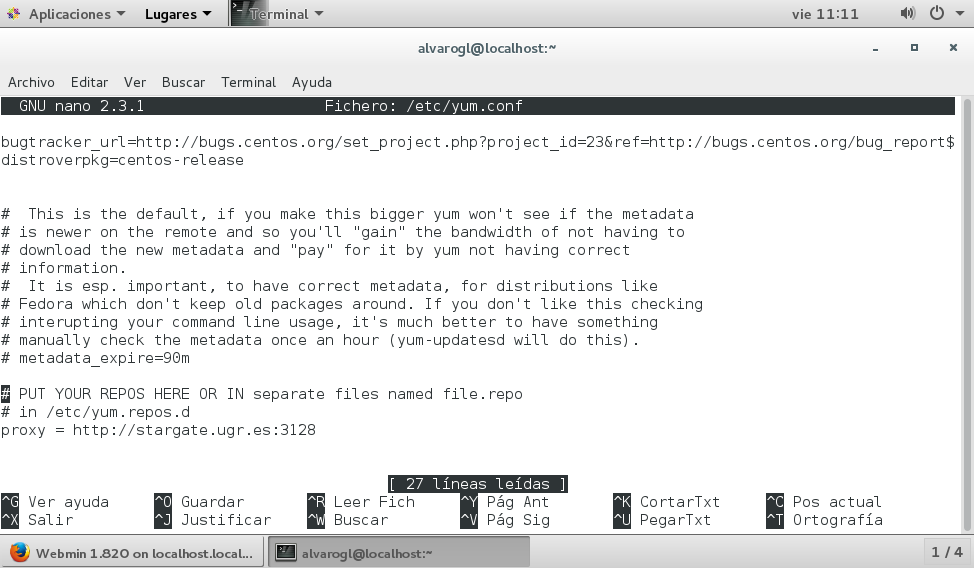
\includegraphics[scale=0.6]{ise2.png}
	\caption{Adición de la sentencia \protect{\textit{proxy = http://stargate.ugr.es:3128}} en \textit{/etc/yum.conf}} \label{ise2}
\end{figure}

\subsection{c) ¿Cómo añadimos un nuevo repositorio?}

Según el manual online de Ubuntu, en \cite{yum-config}, \textit{yum-config-manager} es una orden para administras y configurar algunas opciones de yum. Entre ellas se encuentra la de añadir un repositorio de una dirección URL o de un archivo especificado, además, el repositorio será habilitado.
La sintaxis sería la siguiente:

\begin{verbatim}
yum-config-manager --add-repo=ADDREPO <url o fichero>
\end{verbatim}
\newpage

\section{Cuestión 2.}

\subsection{a) Liste los argumentos de apt necesarios para instalar, buscar y eliminar paquetes.}

Según podemos comprobar en \cite{apt}, apt es un comando que se utiliza para el manejo de paquetes.

\begin{itemize}
	\item{Para instalar paquetes: \begin{verbatim}
		apt install <nombre del paquete o paquetes>
		\end{verbatim}
	}
	\item{Para buscar paquetes: \begin{verbatim}
		apt search <términos de búsqueda>
		\end{verbatim}
		Busca los paquetes que coincidan con los términos de búsqueda.
	}
	\item{Para eliminar paquetes: \begin{verbatim}
		apt remove <nombre del paquete o paquetes>
		\end{verbatim}
		Elimina el paquete o paquetes sin borrar sus ficheros de configuración del sistema.
		Para eliminar estos ficheros de configuración debemos utilizar \textit{purge}, su sintaxis sería la siguiente: \cite{apt-get}
		\begin{verbatim}
		apt purge <nombre del paquete o paquetes>
		\end{verbatim}
	}
\end{itemize}

\subsection{b) ¿Qué ha de hacer para que apt pueda tener acceso a Internet en el PC del aula?(Pistas: archivo de configuración en /etc, proxy: stargate.ugr.es:3128)}

Para ello debemos editar, en este caso, el fichero de configuración de apt en \textit{/etc/apt/apt.conf} como se muestra en \ref{ise3} \cite{proxy-apt} y escribir en él la línea:
\begin{verbatim}
Acquire::http::Proxy "http://stargate.ugr.es:3128"
\end{verbatim}

\begin{figure}[H]
	\centering
	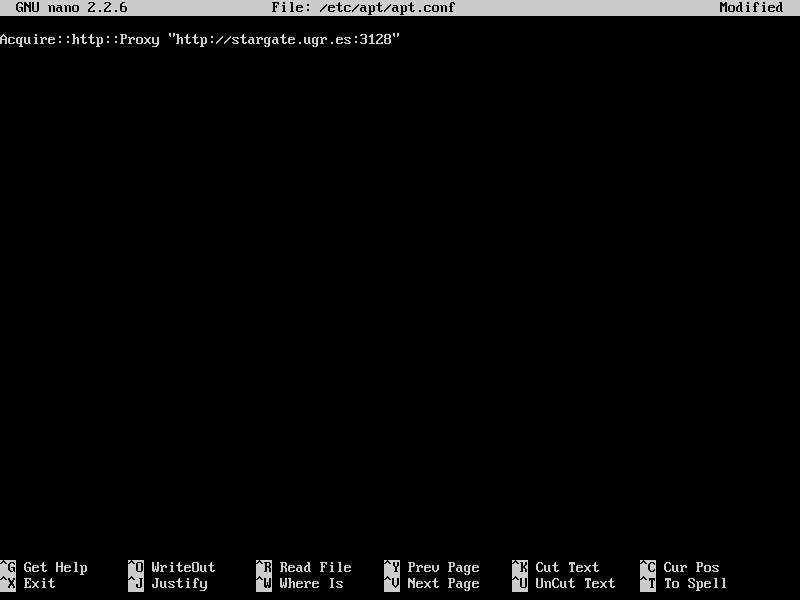
\includegraphics[scale=0.6]{ise3.png}
	\caption{Edición del fichero de configuración de \textit{/etc/apt/apt.conf} con nano} \label{ise3}
\end{figure}

\subsection{c) ¿Cómo añadimos un nuevo repositorio?}

Los repositorios en Ubuntu se almacenan en \textit{/etc/apt/sources.list} o en \textit{/etc/apt/sources.list.d}. Podemos añadir un nuevo repositorio con el comando \textit{add-apt-repository}.
La sintaxis sería:

\begin{verbatim}
add-apt-repository <"repositorio">
\end{verbatim}
\newpage

\section{Cuestión 3.}

\subsection{a) ¿Con qué comando puede abrir/cerrar un puerto usando ufw? Muestre un ejemplo de cómo lo ha hecho}

Según \cite{ufw} y \cite{ufw2}, para abrir un puerto, es decir, para permitir la entrada de paquetes en dicho puerto (cada vez que se diga abrir puertos nos referiremos a esto a lo largo de la memoria), primero debemos habilitar \textit{ufw} de la siguiente forma:

\begin{verbatim}
sudo ufw enable
\end{verbatim}

La sintaxis para habilitar la entrada de paquetes es la siguiente:

\begin{verbatim}
sudo ufw allow <port>/<option: protocol>
\end{verbatim}

Entonces, para habilitar la entrada de paquetes tcp y udp en el puerto 80 escribiríamos en terminal:

\begin{verbatim}
sudo ufw allow 80
\end{verbatim}

Para habilitar entrada de paquetes solo tcp en el puerto 80, como se observa en \ref{ise4}:

\begin{verbatim}
sudo ufw allow 80/tcp
\end{verbatim}

\begin{figure}[H]
	\centering
	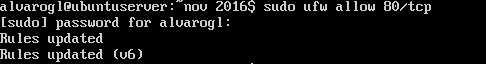
\includegraphics[scale=0.6]{ise4.png}
	\caption{Admisión de la entrada de paquetes tcp en puerto 80} \label{ise4}
\end{figure}

Se procedería de forma análoga para los paquetes udp.
Para rechazar la entrada de paquetes la sintaxis es:

\begin{verbatim}
sudo ufw deny <port>/<optional: protocol>
\end{verbatim}

En \ref{ise5}

\begin{figure}[H]
	\centering
	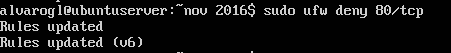
\includegraphics[scale=0.6]{ise5.png}
	\caption{Rechazo de la entrada de paquetes tcp en puerto 80} \label{ise5}
\end{figure}

Su uso es similar al de \textit{ufw allow}

\subsection{b) ¿Con qué comando puede abrir/cerrar un puerto usando firewall-cmd en CentOS? Muestre un ejemplo de cómo lo ha hecho}

Según \cite{firewall-cmd} y \cite{firewall-cmd2}, la sintaxis para abrir puertos en CentOS hay que iniciar \textit{firewall-cmd}, para ello \cite{systemd}:

\begin{verbatim}
systemctl start firewalld.service
\end{verbatim}

Como se nos explica en \cite{systemd}, \textit{systemctl} es el comando principal para controlar e inspeccionar systemd, una suite de gestión y mantenimiento de servicios.

Para abrir puertos en CentOS, la sintaxis es:

\begin{verbatim}
firewall-cmd --zone=<set zone> --add-port=<port>/<optional: protocol>
\end{verbatim}

Se puede añadir la opción \textit{--permanent} para que el puerto permanezca abierto a pesar de reinicios del sistema.

Por, ejemplo, en \ref{ise6} se habilita la entrada de paquetes tcp en el puerto 8080.

\begin{figure}[H]
	\centering
	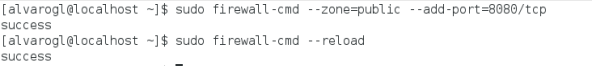
\includegraphics[scale=0.6]{ise6.png}
	\caption{Habilitación de la entrada de paquetes tcp en puerto 8080 y reinicio del servicio firewalld} \label{ise6}
\end{figure}

Después de configurar los puertos, es posible que sea necesario reiniciar el servicio:

\begin{verbatim}
firewall-cmd --reload
\end{verbatim}

De forma análoga, para cerrar puertos:

\begin{verbatim}
firewall-cmd --zone<set zone> --remove-port=<port>/<optional: protocol>
\end{verbatim}

\subsection{c) Utilice el comando nmap para ver que, efectivamente, los puertos están accesibles}

En \cite{nmap} se nos explica cómo se utiliza el comando. Una versión resumida de su sintaxis sería:

\begin{verbatim}
nmap <ip> <optional: -p <port>>
\end{verbatim}

Como se aprecia en \ref{ise7}, he abierto el puerto 10000 para zona pública desde la máquina virtual de la izquierda, a partir de ahora CentOS 3, para escanear el mapa de puertos desde la máquina virtual de la derecha, a partir de ahora CentOS 4.

En CentOS 4, el puerto 10000 aparecía filtrado, pues el servicio estaba en marcha, si bien es cierto que en CentOS 3, el puerto aparecía abierto, pero esta es la máquina local, donde siempre aparecerán abiertos aquellos puertos que utilicen servicios que se estén ejecutando.

Después de habilitar la entrada de datos tcp en CentOS 3 en el puerto 10000, hice un escaneo desde CentOS 4 y el puerto 10000 aparecía abierto.

\begin{figure}[H]
	\centering
	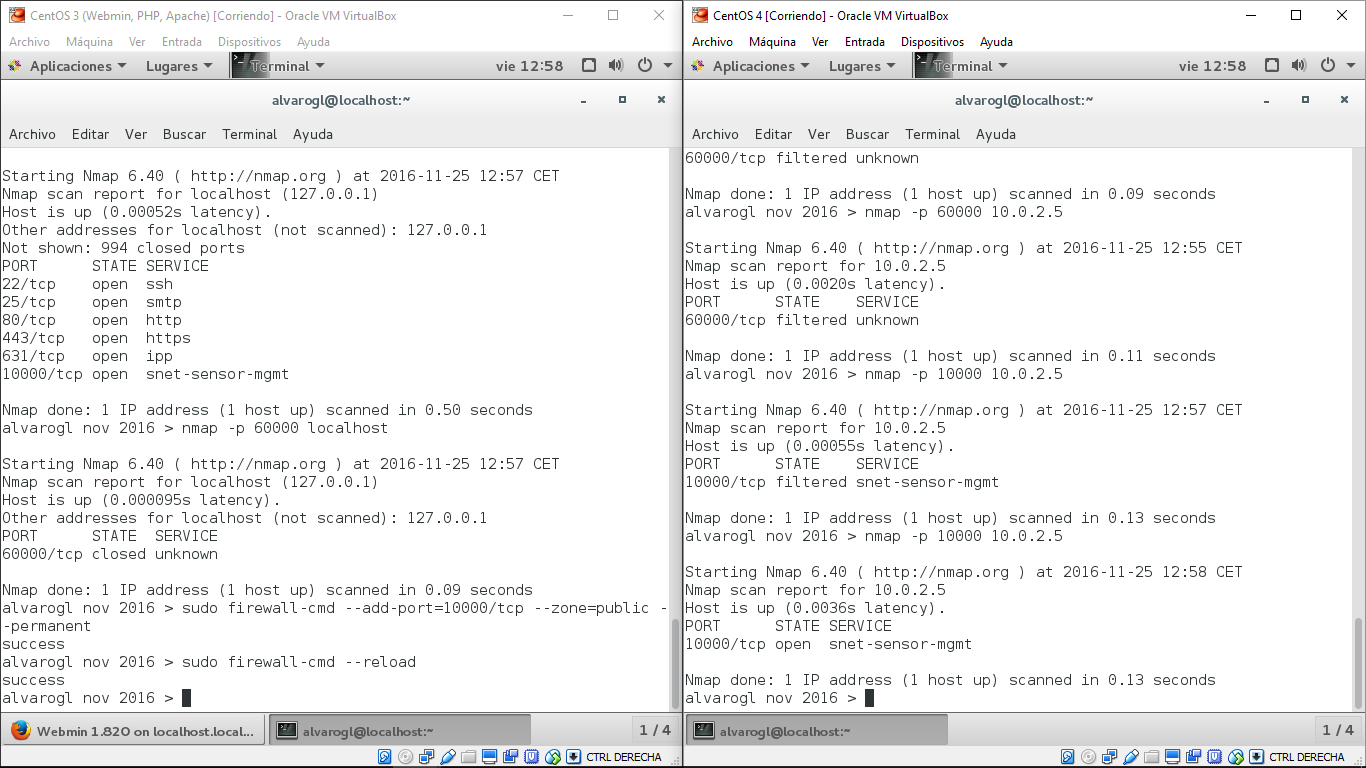
\includegraphics[scale=0.45]{ise7.png}
	\caption{Habilitación de entrada de datos tcp en puerto 10000} \label{ise7}
\end{figure}

\newpage

\section{Cuestión 4. ¿Qué diferencia hay entre telnet y ssh?}

La diferencia principal entre ambos servicios reside en la seguridad. Según \cite{telnet-ssh}, un servidor SSH asegura una conexión segura y encriptada con un cliente SSH. Además, una encriptación fuerte para la autenticación.

En cuanto al protocolo Telnet, habilita una conexión TCP/IP a un servidor. No realiza ningún tipo de encriptación, incluso para la autenticación, pues la contraseña de un usuario se envía en texto plano sin cifrado.


\section{Cuestión 5.}

\subsection{a) ¿Para qué sirve la opción -X?}

Según \cite{ssh} y \cite{x11}, la opción -X sirve para habilitar el redireccionamiento de X11. Esto consiste en que el usuario pueda ejecutar aplicaciones que requieran de entorno gráfico a través de SSH. De esta manera, la aplicación sería ejecutada desde la máquina remota, pero utilizando el servicio de ventanas X11 del usuario local.

\subsection{b) Ejecute remotamente, es decir, desde la máquina anfitriona (si tiene Linux) o desde la otra máquina virtual, el comando gedit en una sesión abierta con ssh. ¿Qué ocurre?}

Al utilizar la opción -X, como podemos ver en \ref{ise8}, se utiliza el servicio de ventanas de la máquina local para ejecutar una aplicación desde la máquina remota y editar un archivo en ella con gedit

\begin{figure}[H]
	\centering
	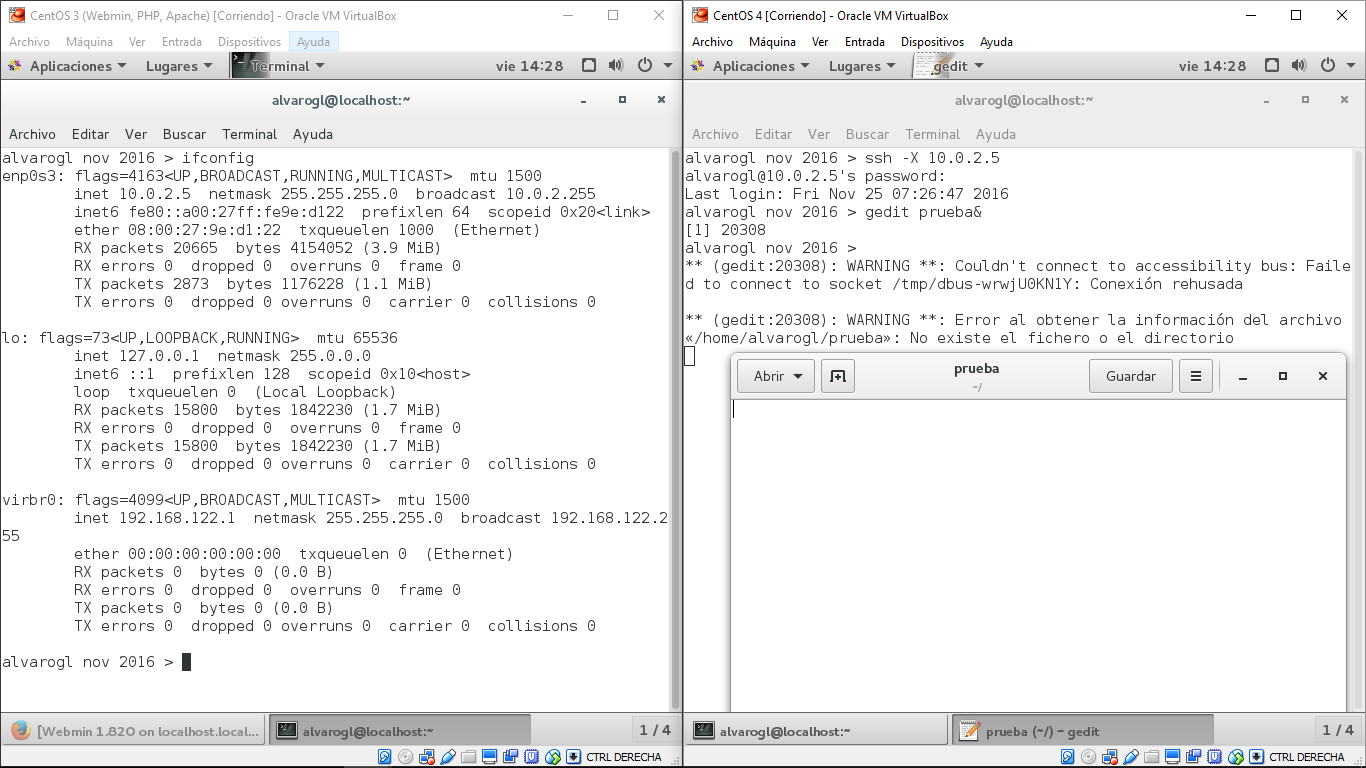
\includegraphics[scale=0.45]{ise8.png}
	\caption{Utilización de \textit{ssh} con redireccionamiento de X11} \label{ise8}
\end{figure}


\section{Cuestión 6. Muestre la secuencia de comandos y las modificaciones a los archivos correspondientes para permitir acceder a la consola remota sin introducir la contraseña. Pruebe que funciona. (Pistas: ssh-keygen, ssh-copy-id)}

Como se nos explica en \cite{ssh-keys}, gracias a ssh-keygen, podemos generar una claves de SSH. Dichas claves se generan por pares, es decir, se genera una clave privada y una clave pública. 
La clave pública se guarda en la ruta \textit{/home/<user>/.ssh/id\_rsa.pub} al ejecutar\begin{verbatim}
ssh-keygen
\end{verbatim} como se muestra en \ref{ise9}.

\begin{figure}[H]
	\centering
	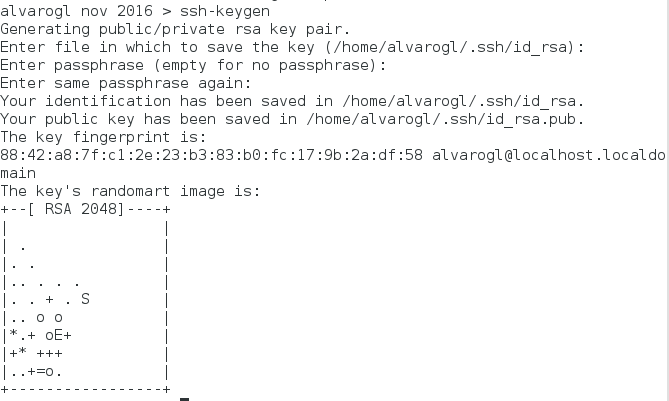
\includegraphics[scale=0.6]{ise9.png}
	\caption{Uso de \textit{ssh-keygen} y \textit{ssh-copy-id} para acceder remotamente por SSH sin contraseña} \label{ise9}
\end{figure}

Después de generar el par de claves, tendremos que copiar la clave pública al servidor remoto para que este pueda conectarse por SSH con autenticación por claves (que no contraseña de caracteres ordinaria). Para ello utilizamos ssh-copy-id:

\begin{verbatim}
ssh-copy-id  
\end{verbatim}

Tras realizar la copia, podemos acceder a la máquina remota sin que se nos pida la contraseña de acceso. Ver \ref{ise10}

\begin{figure}[H]
	\centering
	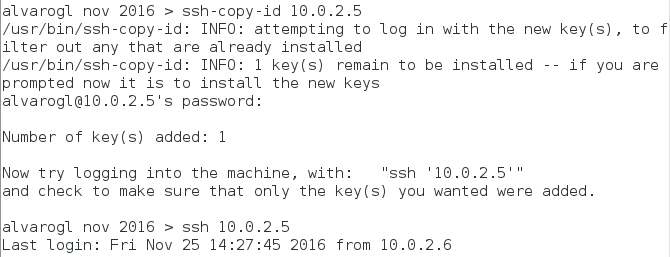
\includegraphics[scale=0.6]{ise10.png}
	\caption{Uso de \textit{ssh-copy-id} y acceso sin contraseña a máquina remota por SSH} \label{ise10}
\end{figure}

\section{Cuestión 7. ¿Qué archivo es el que contiene la configuración del servicio ssh? ¿Qué parámetro hay que modificar para evitar que el usuario root acceda? Cambie el puerto por defecto y compruebe que puede acceder.}

Como podemos comprobar en \cite{ssh-config}, para evitar que el usuario root acceda debemos editar la entrada de \textit{PermitRootLogin}, y para cambiar el puerto por defecto tenemos que cambiar la entrada \textit{Port 22}. Podemos escoger el puerto que queramos mientras no lo ocupe otro servicio, en mi caso escogí el 2345. Las entradas a cambiar quedarían así:

\begin{verbatim}
PermitRootLogin no
Port 2345
\end{verbatim}

El fichero de configuración cambiado se muestra en \ref{ise11}.

\begin{figure}[H]
	\centering
	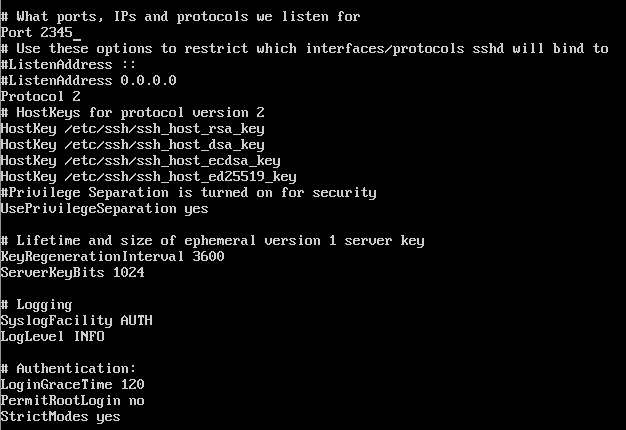
\includegraphics[scale=0.6]{ise11.png}
	\caption{Fichero de configuración \textit{/etc/ssh/sshd\_config} modificado} \label{ise11}
\end{figure}

En \ref{ise12} se comprueba el acceso mediante el nuevo puerto indicado en sshd\_config después de reiniciar el servicio \textit{ssh} utilizando \begin{verbatim}
sudo service ssh restart
\end{verbatim} en Ubuntu Server.

\begin{figure}[H]
	\centering
	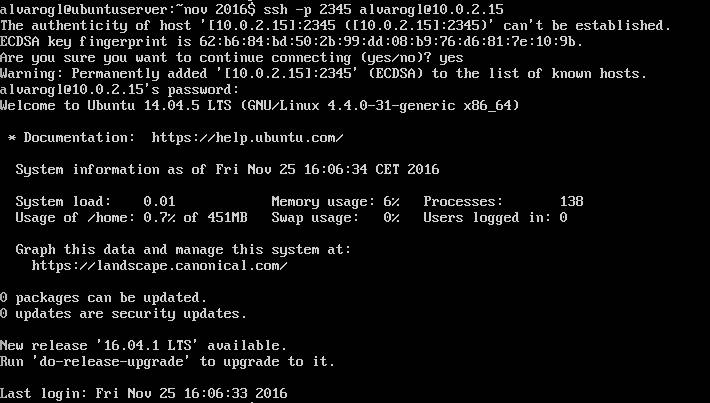
\includegraphics[scale=0.6]{ise12.png}
	\caption{Fichero de configuración \textit{/etc/ssh/sshd\_config} modificado} \label{ise12}
\end{figure}

\section{Cuestión 8. Indique si es necesario reiniciar el servicio ¿Cómo se reinicia un servicio en Ubuntu? ¿Y en CentOS? Muestre la secuencia de comandos para hacerlo.}

Sí. Es necesario en este caso. Pues si no reiniciamos el servicio, \textit{ssh} seguirá ejecutándose en el puerto 22, que es el que tenía por defecto. Para que el servicio se ejecute en el puerto 2345 según la última modificación del fichero de configuración, el servicio debe ser reiniciado.

Para reiniciar servicios en Ubuntu, según \cite{services} debemos ejecutar:

\begin{verbatim}
sudo service <service-name> restart
\end{verbatim}

Ver \ref{ise13}

\begin{figure}[H]
	\centering
	
\includegraphics[scale=0.6]{ise13.png}
	\caption{Reinicio de un servicio en Ubuntu} \label{ise13}
\end{figure}

En CentOS, el equivalente, según \cite{systemd} es:

\begin{verbatim}
sudo systemctl restart <service-name>
\end{verbatim}

Ver \ref{ise14}

\begin{figure}[H]
	\centering
	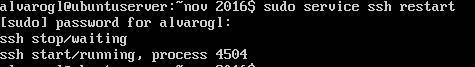
\includegraphics[scale=0.6]{ise14.png}
	\caption{Reinicio de un servicio en CentOS} \label{ise14}
\end{figure}

\section{Cuestión 9. Muestre los comandos que ha utilizado en Ubuntu Server y en CentOS (aunque en este último puede utilizar la GUI, en tal caso, realice capturas de pantalla). Compruebe que la instalación ha sido correcta.}

Según \cite{tasksel}, podemos utilizar el gestor de paquetes tasksel para instalar LAMP si no lo hemos hecho durante la instalación de Ubuntu Server. Esta interfaz nos permite instalar todos los componentes que se nos piden en el ejercicio de una vez:

\begin{verbatim}
sudo tasksel
\end{verbatim}

En CentOS se deben ejecutar las siguientes sentencias según \cite{phpinstall}, \cite{apacheinstall} y \cite{mysqlinstall}:

\begin{verbatim}
sudo yum install httpd
sudo yum install mysql-server
sudo yum install php php-mysql
\end{verbatim}

Para comprobar el correcto funcionamiento de nuestro servidor corriendo con Apache podemos crear un archivo de texto con un mensaje de prueba en \textit{/var/www/html/index.html} y acceder a localhost desde un navegador o http:://<IP> desde una máquina remota. En \ref{ise15} se muestra en buen funcionamiento el servidor de apache2.

\begin{figure}[H]
	\centering
	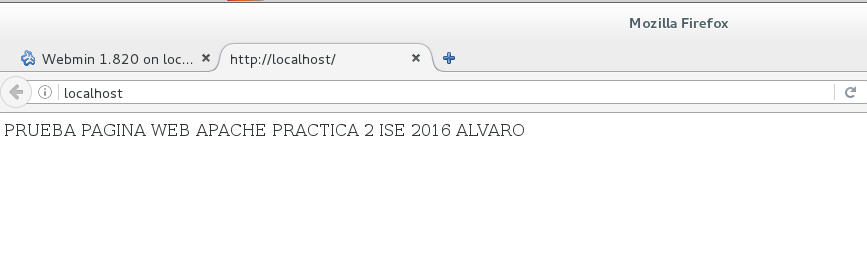
\includegraphics[scale=0.6]{ise15.png}
	\caption{Comprobación de servidor apache2 corriendo en CentOS} \label{ise15}
\end{figure}

\begin{figure}[H]
	\centering
	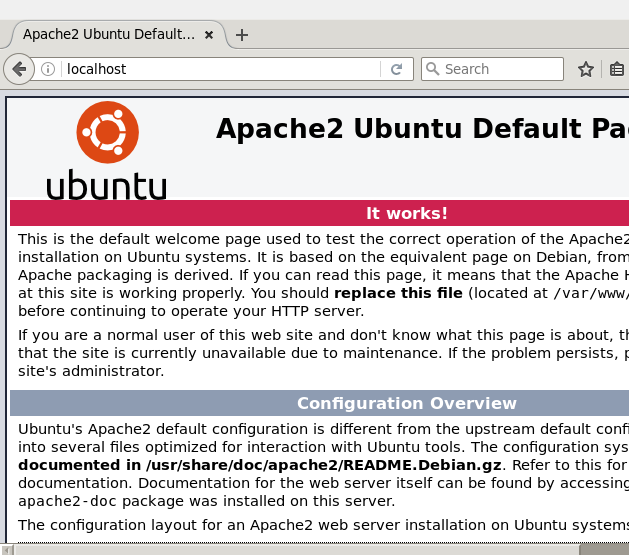
\includegraphics[scale=0.6]{ise16.png}
	\caption{Comprobación de servidor apache2 corriendo en Ubuntu} \label{ise16}
\end{figure}

Para comprobar que se han instalado php y mysql basta con ejecutar\ref{ise17}:

\begin{verbatim}
php --version
mysql --version
\end{verbatim}

\begin{figure}[H]
	\centering
	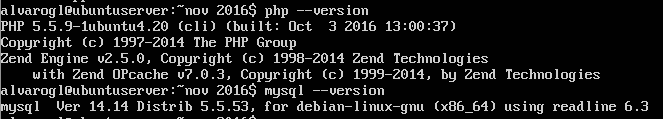
\includegraphics[scale=0.6]{ise17.png}
	\caption{Comprobación de que PHP y MySQL están instalados} \label{ise17}
\end{figure}

\section{Cuestión 10. Realice la instalación usando GUI o PowerShell y compruebe que el servicio está funcionando accediendo a la MV a través de la anfitriona}

Para instalar IIS seguimos los pasos indicados en el guión de prácticas. Buscamos la aplicación IIS y la iniciamos, como se observa en \ref{ise18} \cite{iis}

\begin{figure}[H]
	\centering
	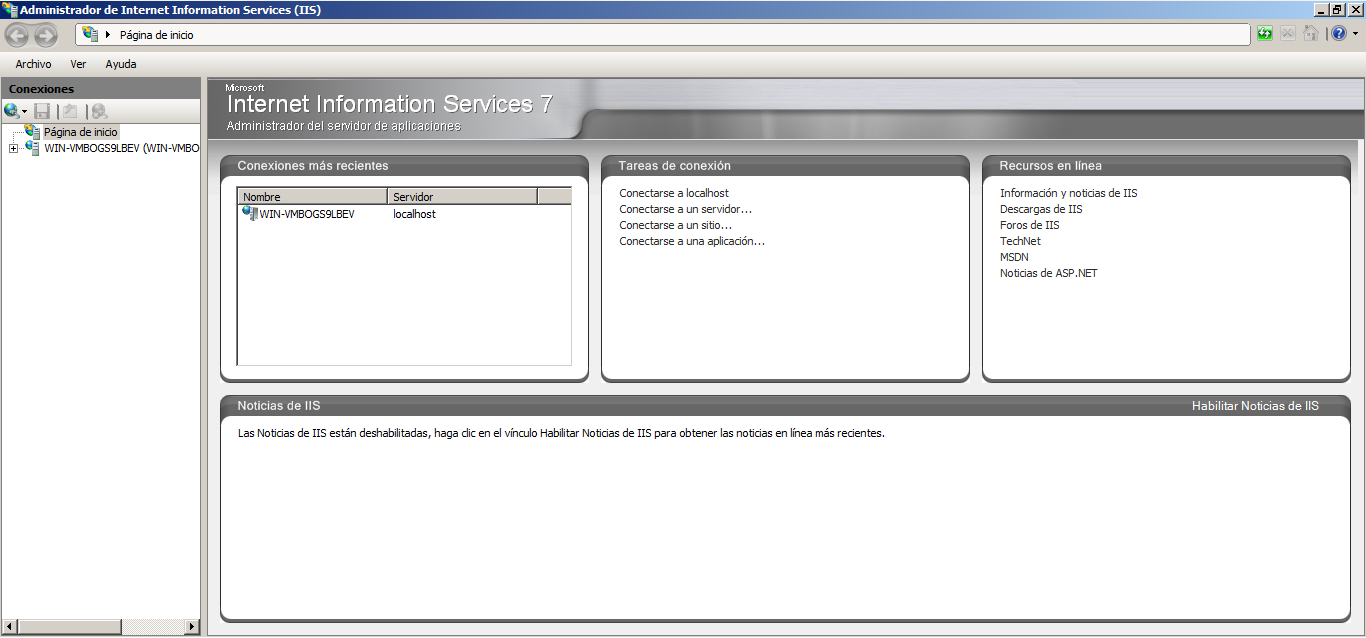
\includegraphics[scale=0.45]{ise18.png}
	\caption{Ejecución de IIS} \label{ise18}
\end{figure}

En \ref{ise20} se muestra la IP de la máquina virtual

\begin{figure}[H]
	\centering
	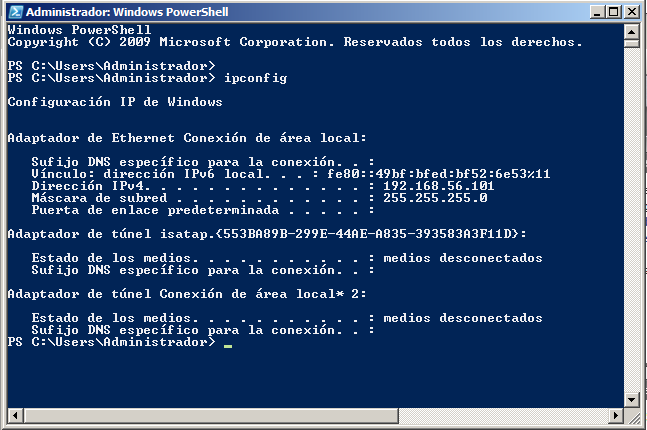
\includegraphics[scale=0.6]{ise20.png}
	\caption{Salida ipconfig máquina virtual} \label{ise20}
\end{figure}

En \ref{ise19} se muestra el acceso exitoso desde la máquina anfitriona al servidor IIS.

\begin{figure}[H]
	\centering
	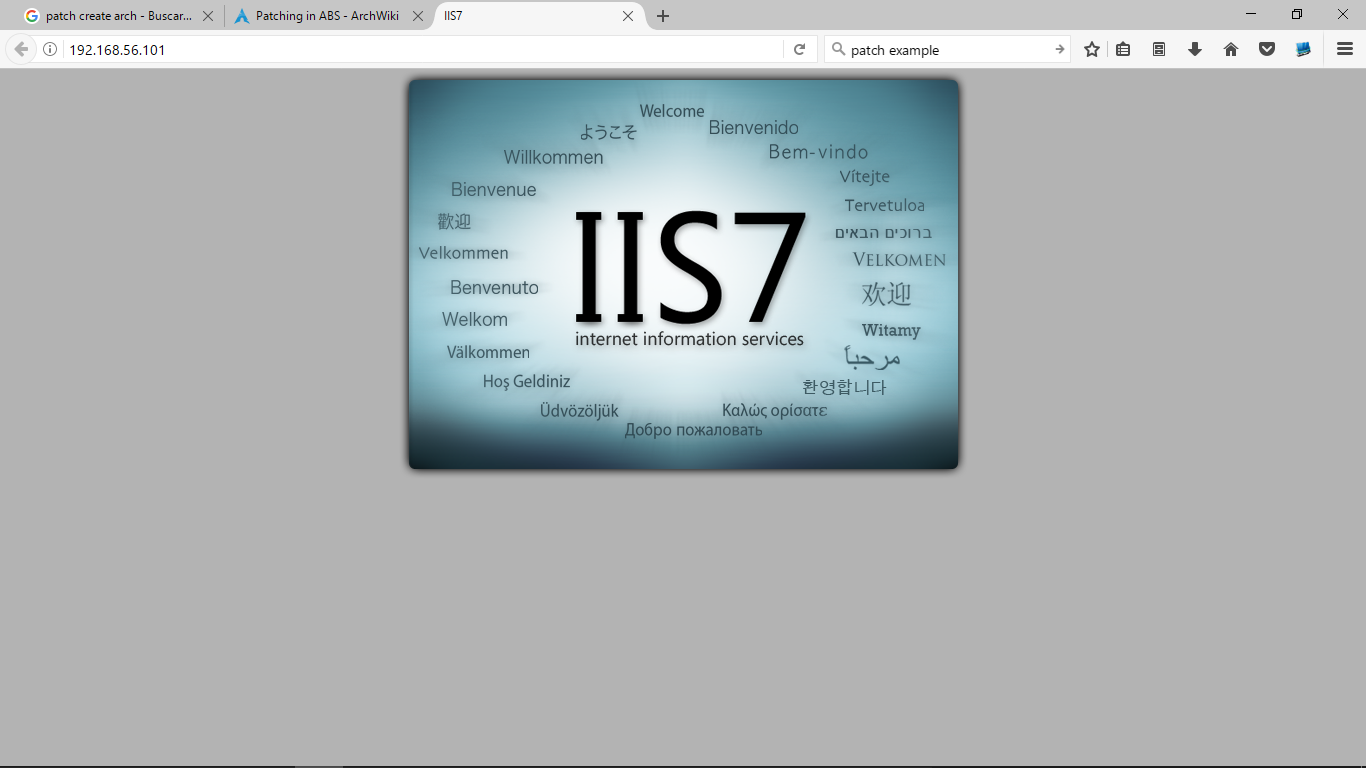
\includegraphics[scale=0.45]{ise19.png}
	\caption{Acceso desde máquina anfitriona a IIS} \label{ise19}
\end{figure}

Para que el acceso se produzca satisfactoriamente la máquina virtual debe estar configurada con una conexión host-only.

\section{Cuestión 11. Muestre un ejemplo de uso del comando (p.ej. http://fedoraproject.org/wiki/VMWare)}

En \cite{patch} se nos enseña a utilizar este útil comando de Linux.

Para mostrar un ejemplo de su uso, creamos un archivo sum.cpp. Supongamos que este tiene un fallo, como se puede apreciar en \ref{ise21}.

\begin{figure}[H]
	\centering
	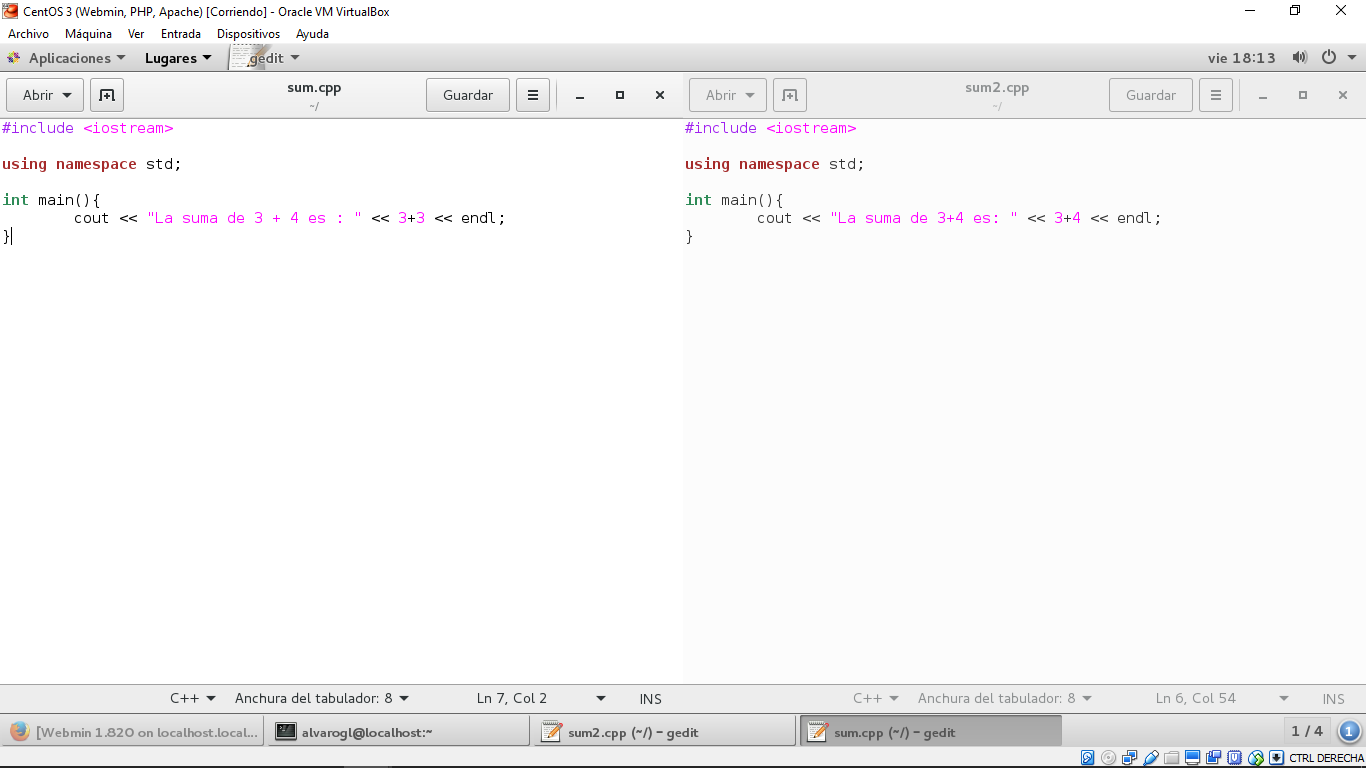
\includegraphics[scale=0.45]{ise21.png}
	\caption{Archivos sum.cpp y sum2.cpp (sum.cpp corregido)} \label{ise21}
\end{figure}

Creamos el parche y lo aplicamos:

\begin{verbatim}
diff sum.cpp sum2.cpp > p.patch
patch sum.cpp p.patch
\end{verbatim}

\begin{figure}[H]
	\centering
	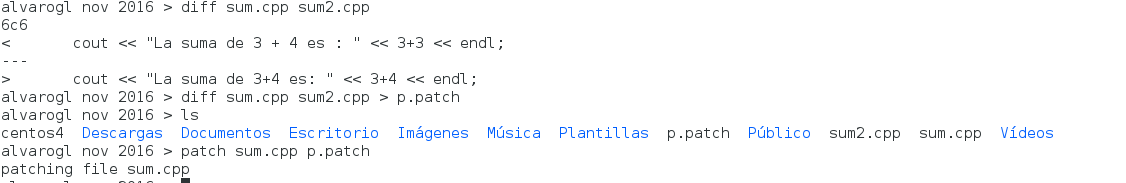
\includegraphics[scale=0.6]{ise22.png}
	\caption{Creación y aplicación del parche} \label{ise22}
\end{figure}

En \ref{ise23} se muestra el resultado final de sum.cpp, ya habiendo aplicado el parche sobre él, de forma que hemos conseguido corregirlo.

\begin{figure}[H]
	\centering
	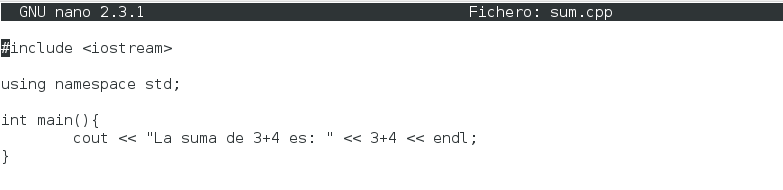
\includegraphics[scale=0.6]{ise23.png}
	\caption{Resultado final del archivo} \label{ise23}
\end{figure}

\section{Cuestión 12. Realice la instalación de esta aplicación y pruebe a modificar algún parámetro de algún servicio. Muestre las capturas de pantalla pertinentes así como el proceso de instalación.}

Webmin está disponible en \cite{webmin}

\begin{figure}[H]
	\centering
	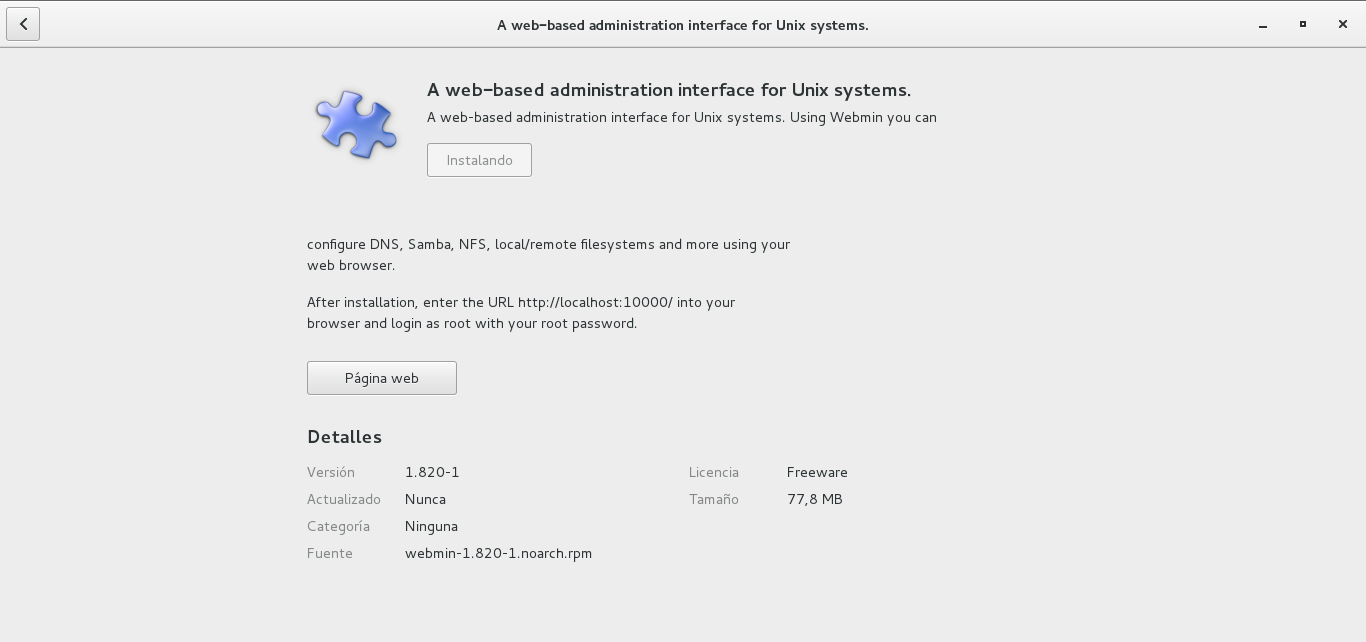
\includegraphics[scale=0.45]{instalacionwebmin.png}
	\caption{Instalación de webmin con interfaz gráfica} \label{instalacionwebmin}
\end{figure}

Accedemos a webmin a través de localhost:10000 en un navegador \ref{interfazwebmin}.

\begin{figure}[H]
	\centering
	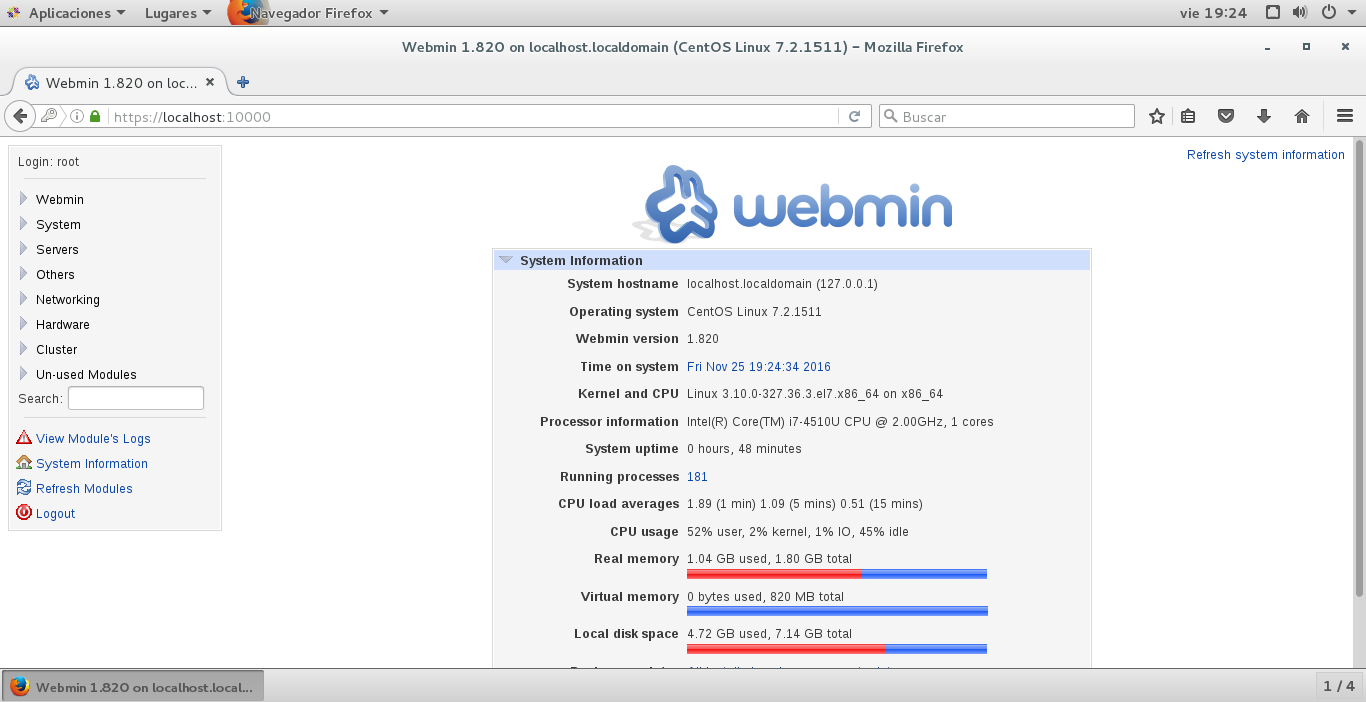
\includegraphics[scale=0.45]{webmin-interfaz.png}
	\caption{Interfaz de webmin} \label{interfazwebmin}
\end{figure}

En mi caso, he probado el \textit{shell} de comandos, como se puede ver en \ref{shell-prueba-cpuinfo} para ver información sobre la CPU.

\begin{figure}[H]
	\centering
	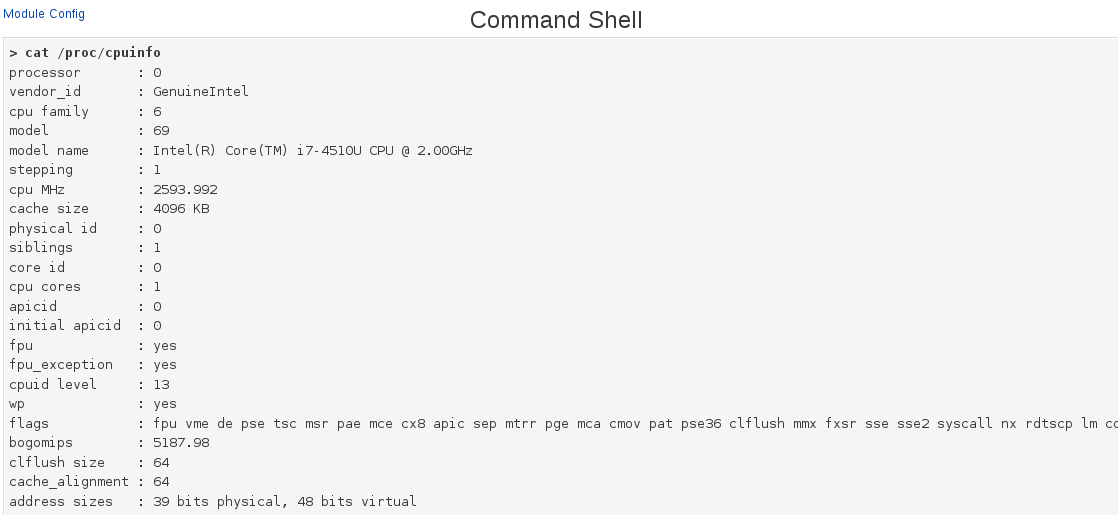
\includegraphics[scale=0.45]{shell-prueba-cpuinfo.png}
	\caption{Interfaz de webmin} \label{shell-prueba-cpuinfo}
\end{figure}

También he creado una nueva tarea para que el demonio cron la ejecute de manera semanal para comprobar el espacio disponible en las particiones, y que esta información se almacene en \textit{/var/log/weeklyscan.log} (ver \ref{cron-job})
	
\begin{figure}[H]
	\centering
	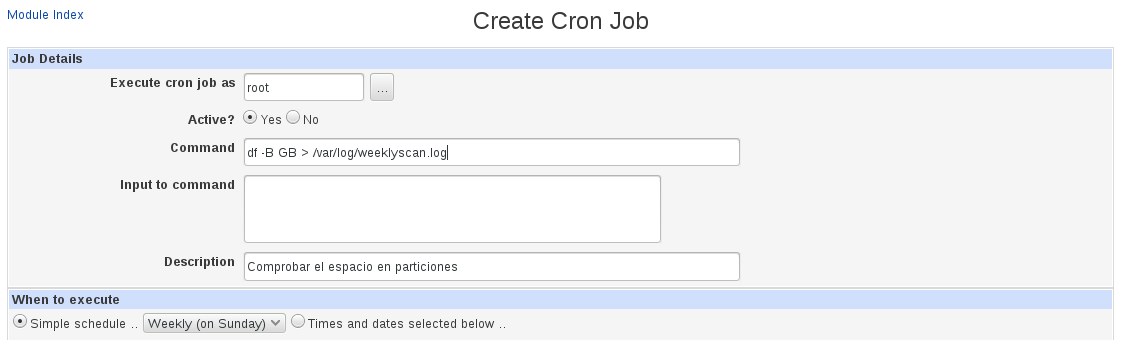
\includegraphics[scale=0.45]{cron-job.png}
	\caption{Creación de una nueva tarea de cron} \label{cron-job}
\end{figure}

\section{Cuestión 13. Instale phpMyAdmin, indique cómo lo ha realizado y muestre algunas capturas de pantalla. Configure PHP para poder importar BDs de hasta 25MiB (en vez de los 8 MiB de límite por defecto). Indique cómo ha realizado el proceso y muestre capturas de pantalla.}

Para instalar phpmyadmin ejecutamos:

\begin{verbatim}
sudo apt install phpmyadmin
\end{verbatim}

En \ref{installphpmyadmin} aparece la interfaz de instalación de phpmyadmin.

\begin{figure}[H]
	\centering
	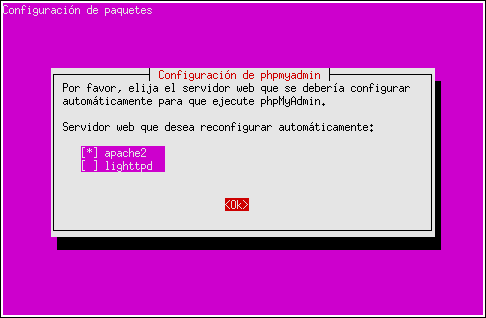
\includegraphics[scale=0.6]{installphpmyadmin.png}
	\caption{Instalación de phpmyadmin} \label{installphpmyadmin}
\end{figure}

Según \cite{php}, donde se nos describen todas las entradas del fichero php.ini de \textit{/etc/php5/apache2/php.ini} y cómo afectan las modificaciones de dicho archivo de configuración al servidor, podemos cambiar el tamaño máximo de datos de POST permitidos. Debemos cambiar el valor antiguo de \textit{post\_max\_size} por '25M' como se muestra en \ref{editphpini} dicho valor debe ser mayor que \textit{ upload\_max\_filesize}. \textit{memory\_limit} debe ser mayor que \textit{post\_max\_size}. Comprobamos que se cumplen estas dos restricciones y salvamos el archivo.

\begin{figure}[H]
	\centering
	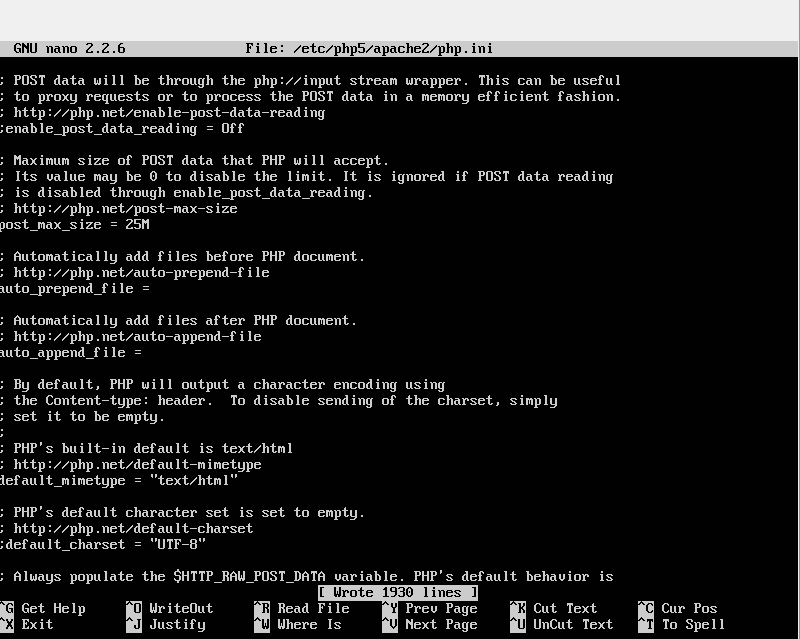
\includegraphics[scale=0.6]{editphpini.png}
	\caption{Edición de \textit{/etc/php5/apache2/php.ini}} \label{editphpini}
\end{figure}

\section{Cuestión 14. Viste al menos una de las webs de los software mencionados y pruebe las demos que ofrecen realizando capturas de pantalla y comentando qué está realizando}

En mi caso, he visitado la web de ISPConfig, la interfaz se muestra en \ref{ispconfig-demo}. He accedido con las credenciales de la demo para probar el software.

\begin{figure}[H]
	\centering
	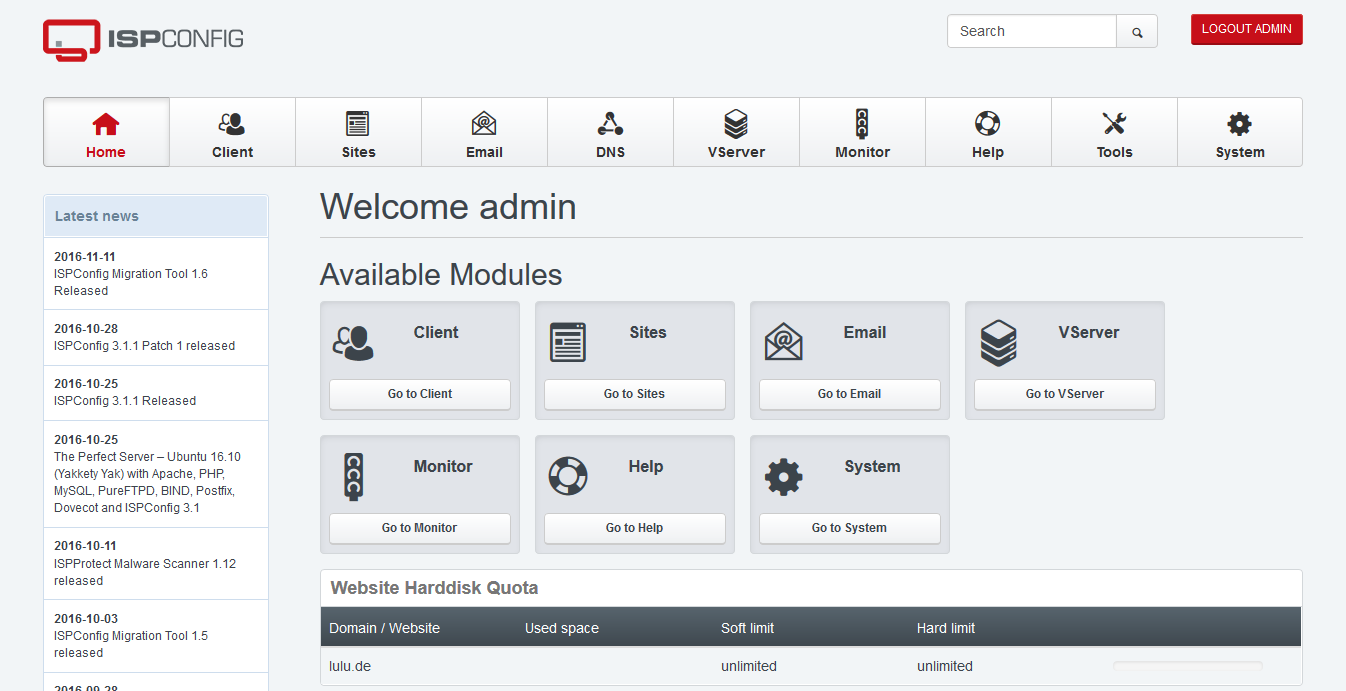
\includegraphics[scale=0.45]{ispconfig-demo.png}
	\caption{Pantalla de bienvenida al administrador de Webmin} \label{ispconfig-demo}
\end{figure}

He creado un nuevo usuario para bases de datos (Ver \ref{nuevo_usuario_bd}) para después crear una base de datos nueva (Ver \ref{creando-bd}).

\begin{figure}[H]
	\centering
	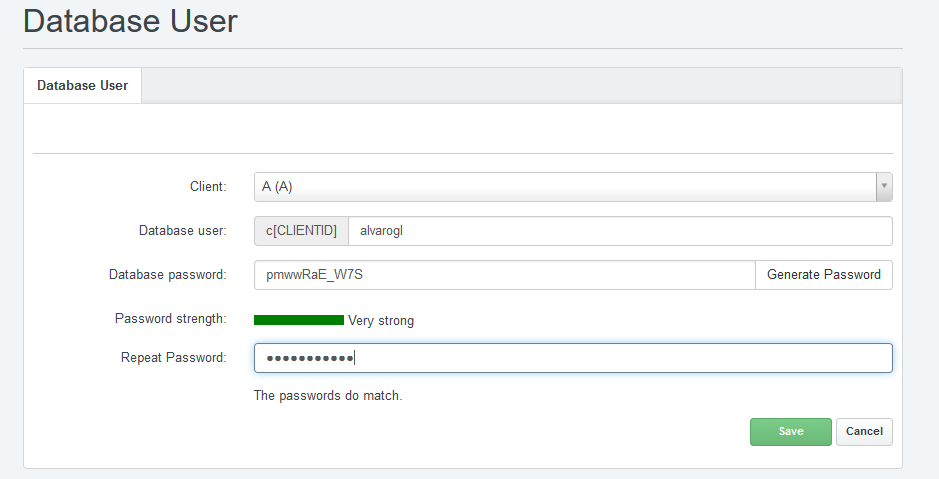
\includegraphics[scale=0.6]{nuevo-usuario-bd.png}
	\caption{Nuevo usuario para bases de datos} \label{nuevo_usuario_bd}
\end{figure}

\begin{figure}[H]
	\centering
	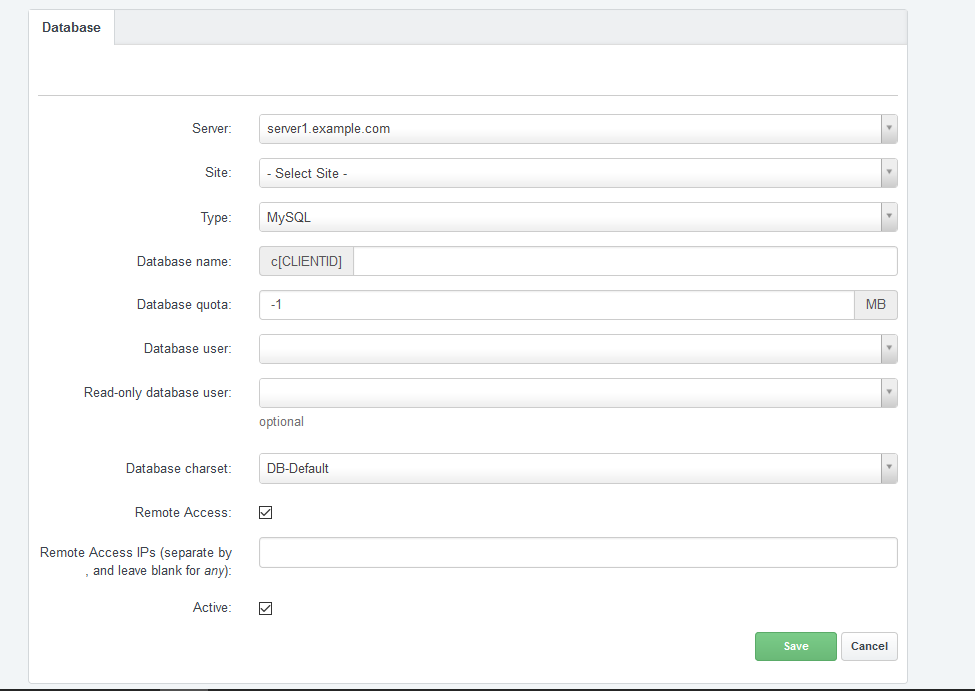
\includegraphics[scale=0.6]{creando-bd.png}
	\caption{Nueva base de datos} \label{creando-bd}
\end{figure}

Algunas herramientas interesantes de administración del servidor se pueden apreciar en \ref{herramientas-interesantes}, entre las que destaco las de mostrar la carga del servidor, la utilización del disco, el uso de memoria y los servicios activos.

\begin{figure}[H]
	\centering
	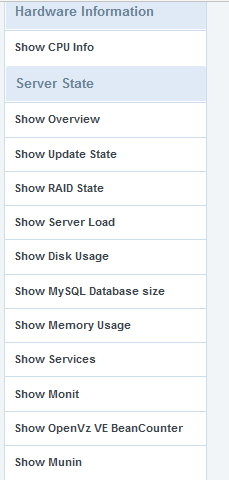
\includegraphics[scale=0.6]{herramientas-interesantes.png}
	\caption{Herramientas interesantes} \label{herramientas-interesantes}
\end{figure}

Me hubiera gustado probar más características de esta herramienta, pero la versión demo limita mucho la funcionalidad de la misma.

\section{Cuestión 15.}

\subsection{a) Ejecute los ejemplos de find, grep}

En \ref{grepfirefox} se aprecia el ejemplo de \textit{grep} del guión de prácticas ejecutado:

\begin{verbatim}
ps -Af | grep firefox
\end{verbatim}

\begin{figure}[H]
	\centering
	
\includegraphics[scale=0.6]{grepfirefox.png}
	\caption{Ejecución del comando \protect{\textit{ps -Af | grep firefox}}} \label{grepfirefox}
\end{figure}

Para el ejemplo de \textit{find}, ejecutamos en el directorio que aparece en \ref{archivosfind} el comando(Ver \ref{findexec}):

\begin{verbatim}
find -name 'test*' -exec cp {} ~/tests \
\end{verbatim}

\begin{figure}[H]
	\centering
	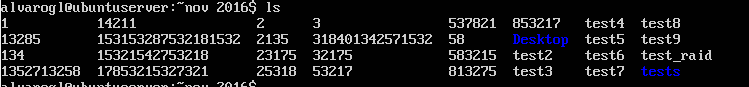
\includegraphics[scale=0.6]{archivosfind.png}
	\caption{Archivos en el directorio antes de la ejecución} \label{archivosfind}
\end{figure}

\begin{figure}[H]
	\centering
	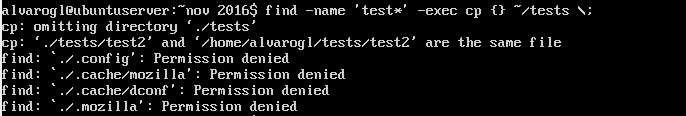
\includegraphics[scale=0.6]{findexec.png}
	\caption{Ejecución del comando} \label{findexec}
\end{figure}

Los errores que se aprecian en \ref{findexec} salen porque hay archivos que el sistema no permite copiar sin permisos de root.

El resultado de la ejecución puede verse en \ref{resultado}. Todos los archivos que comienzan por test han sido transferidos al directorio indicado.

\begin{figure}[H]
	\centering
	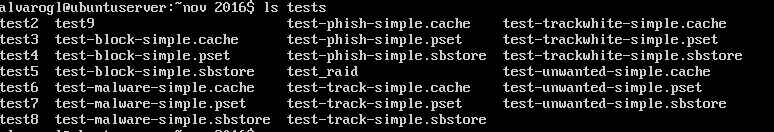
\includegraphics[scale=0.6]{resultado.png}
	\caption{Resultado de la ejecución} \label{resultado}
\end{figure}


\subsection{b) Escriba el script que haga uso de sed para cambiar la configuración de ssh y reiniciar el servicio}

Vamos a realizar el script que se pide en el guión de prácticas, cuya ejecución brindará acceso a usuarios por autenticación con contraseña al servidor por unos segundos.

Según \ref{sed-script}, podemos modificar un archivo \textit{'in-place'} con la opción -i de sed. 
Con el comando `s' los caracteres entre / son reemplazados por los que se encuentran detrás de la segunda /.
Con el comando `g' los espacios son tenidos en cuenta.

El script \ref{sed-script} primero modifica con sed el archivo de configuración de ssh para proporcionar el acceso con contraseña, después espera 30 segundos, vuelve a dejar el fichero de configuración en su estado original con sed, y finalmente reinicia el servicio\cite{sed}.

\begin{figure}[H]
	\centering
	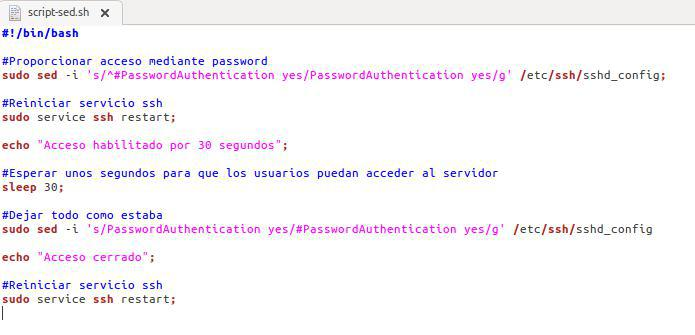
\includegraphics[scale=0.6]{sed-script.png}
	\caption{Script de sed en bash} \label{sed-script}
\end{figure}

Probamos el funcionamiento del script, comprobando antes, durante, y después de la ejecución del mismo el estado del fichero de configuración de \textit{ssh} como se puede ver en \ref{sed-script-prueba}.

\begin{figure}[H]
	\centering
	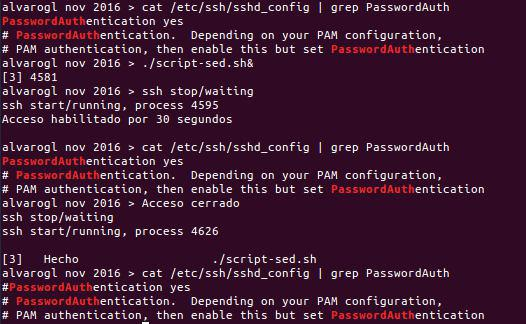
\includegraphics[scale=0.6]{sed-script-prueba.png}
	\caption{Resultado de la ejecución del script y comprobación de su funcionamiento} \label{sed-script-prueba}
\end{figure}

El script será añadido al archivo comprimido de la entrega de la práctica.

\subsection{c) Muestre un ejemplo de uso para awk}

En \cite{awk} se nos explica el uso del comando \textit{awk}. Es muy útil para la manipulación de textos.

En el siguiente ejemplo, \textit{awk} toma los valores de las columnas que le indicamos y las imprime.
Supongamos que tenemos un fichero con las notas de ISE de cada práctica como en \ref{notas-ise} se muestra.

\begin{figure}[H]
	\centering
	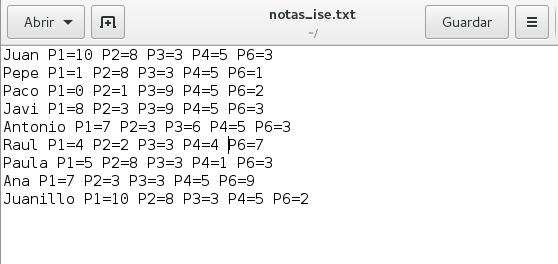
\includegraphics[scale=0.6]{notas-ise.png}
	\caption{Fichero inicial} \label{notas-ise}
\end{figure}

Resulta que solo queremos saber las notas de las prácticas 1 y 2. Entonces ejecutamos el siguiente comando:

\begin{verbatim}
awk '/a {$1 "\t" $2 "\t" $3 notas_ise.txt}}
\end{verbatim}

El resultado de la ejecución se muestra en \ref{notas-ise-final}.

\begin{figure}[H]
	\centering
	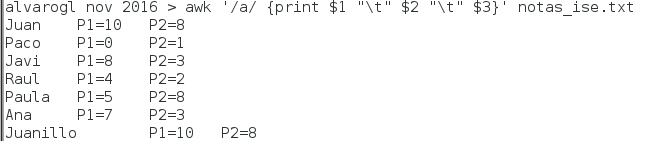
\includegraphics[scale=0.6]{notas-ise-final.png}
	\caption{Resultado de la ejecución del comando} \label{notas-ise-final}
\end{figure}

\section{Cuestión 16. Escriba el script para cambiar el acceso a ssh usando PHP o Python}

En \cite{python} se explica cómo abrir, leer y escribir ficheros en Python, una guía útil para confeccionar el script que se pide, como se puede ver en \ref{sed-script}.

\begin{figure}[H]
	\centering
	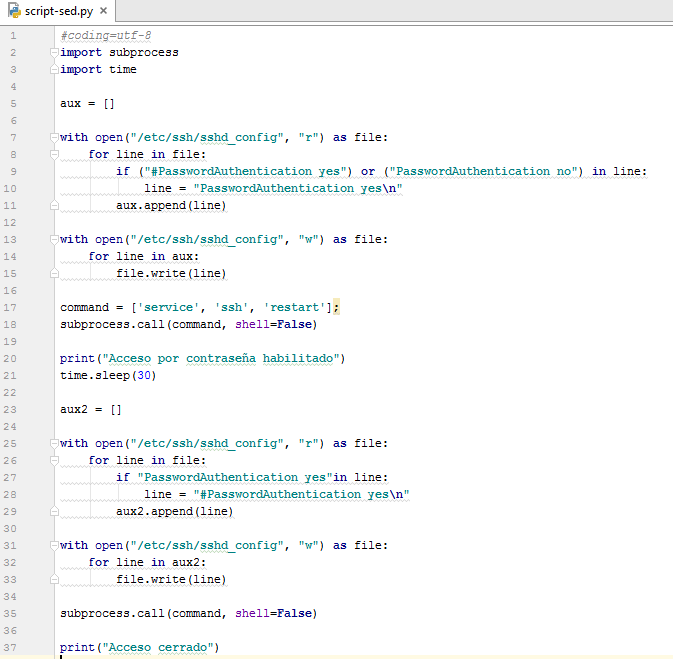
\includegraphics[scale=0.6]{sed-scriptpy.png}
	\caption{Script en Python para modificar la configuración de ssh} \label{sed-scriptpy}
\end{figure}

Probamos el funcionamiento del script, comprobando antes, durante, y después de la ejecución del mismo el estado del fichero de configuración de \textit{ssh} como se puede ver en \ref{sed-scriptpy-prueba}.

\begin{figure}[H]
	\centering
	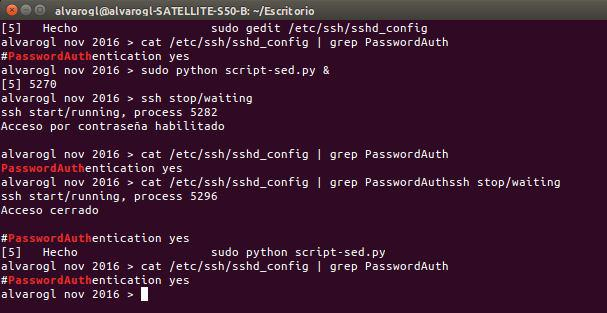
\includegraphics[scale=0.6]{sed-scriptpy-prueba.png}
	\caption{Resultado de la ejecución del script y comprobación de su funcionamiento} \label{sed-scriptpy-prueba}
\end{figure}

El script será añadido al archivo comprimido de la entrega de la práctica.

\section{Cuestión 17. Abra una consola de PowerShell y pruebe a parar un programa en ejecución (p.ej), realice capturas de pantalla y comente lo que muestra}

Abrimos un programa cualquiera, por ejemplo el Bloc de Notas, como se muestra en \ref{notepad-abierto}.

\begin{figure}[H]
	\centering
	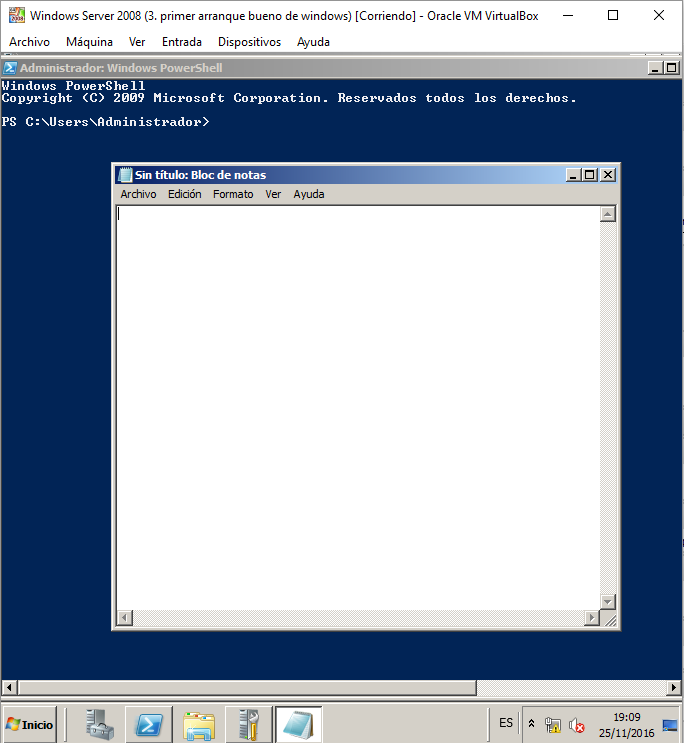
\includegraphics[scale=0.6]{notepad-abierto.png}
	\caption{Programa Notepad abierto} \label{notepad-abierto}
\end{figure}

Mostramos los procesos en ejecución como podemos ver en \ref{procesos-ejecucion} con:

\begin{verbatim}
Get-Process
\end{verbatim}

\begin{figure}[H]
	\centering
	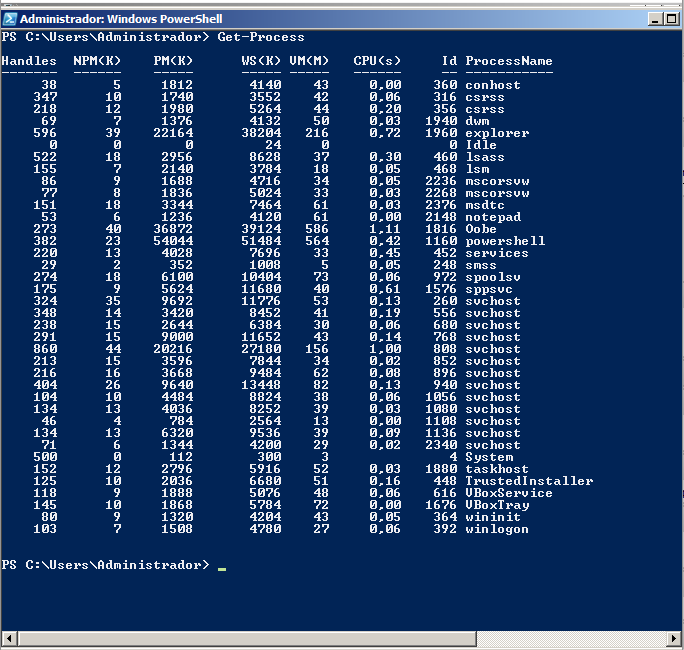
\includegraphics[scale=0.6]{procesos-ejecucion.png}
	\caption{Procesos en ejecución} \label{procesos-ejecucion}
\end{figure}

Por último, identificamos el proceso que queremos matar y ejecutamos (ver \ref{stopnote}):

\begin{verbatim}
Stop-Service notepad
\end{verbatim}

\begin{figure}[H]
	\centering
	
\includegraphics[scale=0.6]{stopnote.png}
	\caption{Ejecución de \textit{Stop-Process -Name notepad}} \label{stopnote}
\end{figure}

\section{Opinión sobre la práctica}
En mi opinión, esta práctica ha sido muy extensa. Personalmente, he ido muy justo para entregarla porque requiere de mucho tiempo para hacer muchas capturas de pantalla, instalar y descargar muchos programas y me parece más compleja que la primera práctica y no me ha dado tiempo a hacer ninguna pregunta opcional.
Si bien es cierto que es posible que sea mejor así, ya que las últimas prácticas coinciden con épocas en las que hay muchos exámenes y hay más carga lectiva de lo normal. Así que no me parece mal que se realice una práctica de tal densidad al principio-mitad de curso como se viene haciendo.
Sugeriría que se pudieran entregar las preguntas opcionales hasta final de curso, si no se ha contemplado ya esto.

\newpage
\bibliographystyle{plain}
\bibliography{biblio}

\end{document}